\documentclass[a4paper, 12pt]{article}
%\usepackage[utf8]{inputenc} 
\usepackage[frenchb]{babel}
\usepackage{fullpage}
\usepackage[T1]{fontenc} 
\usepackage{graphicx}  
\usepackage[final]{pdfpages}
\usepackage{amsmath, amssymb,amsthm}
\usepackage{algorithm,algorithmic}
\usepackage{listingsutf8}
\usepackage{lmodern}
\usepackage{tikz}
\usepackage{pgfplots}

\newtheorem{mydef}{Définition}
\newtheorem{thm}{Théorème}
\newtheorem{lem}{Lemme}
\newtheorem{cor}{Corollaire}
\newtheorem{prop}{Propriété}

\title{Rapport de Méthodes approchées.}
\author{Dyce William, Loukil Amal, Ouazzani-chahdi Sabrina : \\ M1 MOCA}
\date{semestre 2 : 2011-2012}

\begin{document} 

\maketitle

\begin{abstract}
  Le présent document consiste en un mémoire au sujet
  d'exercices à la fois théoriques et pratiques sur diverses
  problèmatiques liées à l'étude de méthodes approchées pour la
  résolution de problèmes NP-difficiles. 
\end{abstract}
\vspace{2cm}
\textit{Travelling salesman's problem :}
\begin{figure}[h!]
\centering
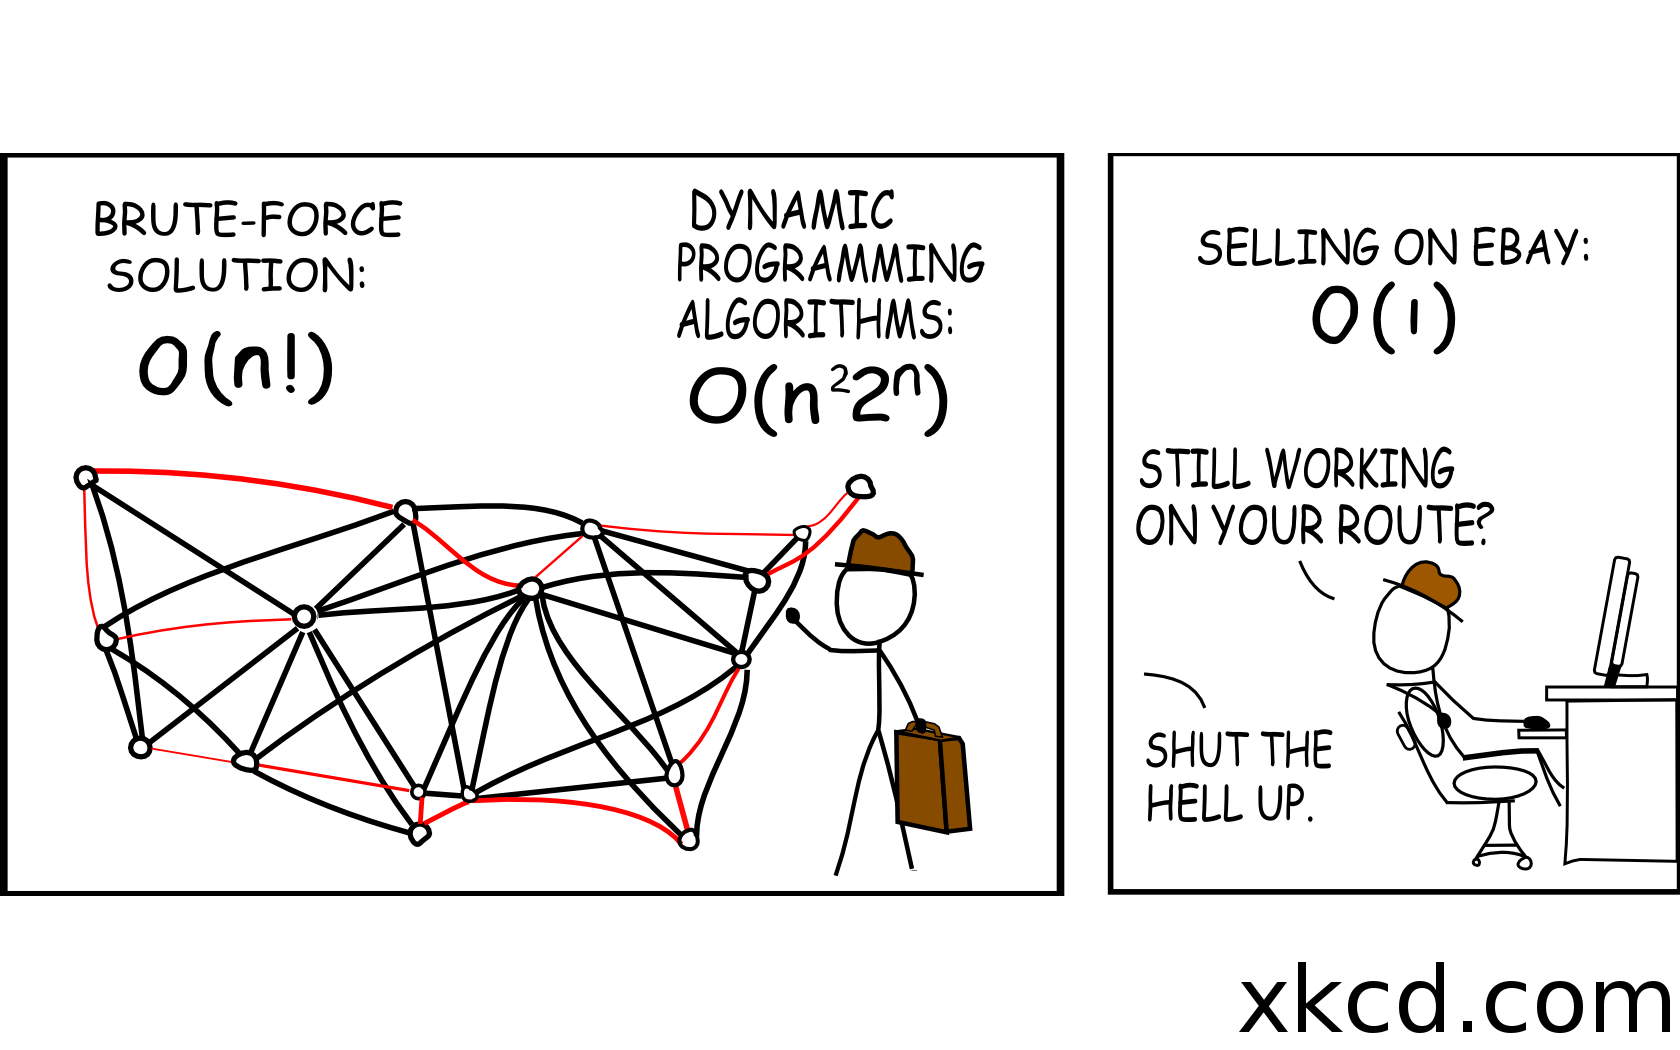
\includegraphics[height = 9cm]{commerce.png}
\end{figure}


\pagebreak

\tableofcontents

\pagebreak

\listoffigures

\listoftables
\pagebreak

\section{Généralités et notations}

\pagebreak

\section{Partie théorique}

\subsection{Programmation linéaire en nombres entiers}

\subsubsection*{Exercice 1}

\paragraph{Question 1}

\begin{itemize}
\item[] a) Le programme linéaire en nombre entier présenté dans
  l'énoncé se justifie de la manière suivante~:
\begin{itemize}
\item $x_j \in \{0,1\}, j=1..n$ car on a le choix binaire entre prendre un
  sommet (donc le compter avec 1), ou ne pas le prendre (ne pas le
  compter avec 0, élement neutre de l'addition). Il y a bien
  évidemment n sommets, d'où l'indexation de 1 à n.
\item $min z = \sum^n _{i=1} x_i$ car on souhaite minimiser le nombre
  de sommets pris.
\item $x_r + x_s \geq 1$ car au moins un sommet doit être pris pour
  couvrir une arête.
\end{itemize}
Ces trois conditions décrivent donc bien le problème de la couverture minimale.
\item[] b) exemple du triangle (à faire en dessin), cette condition
  n'est donc pas suffisante.
\item[] c) Montrons par l'absurde que le programme linéaire en nombres
  entiers est une borne inférieure de toute solution optimale.
\begin{proof}
Supposons que pour une instance donnée, on ait une solution optimale
de vertex cover qui soit meilleure que PLNE. Cela veut donc dire que
PLNE garde au au moins un sommet <<~en trop~>>. Or PLNE devrait
minimiser le nombre de sommets et le simplexe est adéquat. Le résultat
est donc absurde et contredit notre hypothèse de départ.
\end{proof}
\item[] d) Nous allons ici montrer de deux manières différentes que la
  relaxation des contraintes d'intégrité implique $x_r \geq
  \frac{1}{2}$ ou $x_s \geq \frac{1}{2}$.
\begin{itemize}
\item Première démonstration.
\begin{proof}
On veut, malgré la relaxation des contraintes d'intégrité, conserver
l'inégalité $x_r + x_s \geq 1$. Ainsi, on a $\neg (x_r + x_s < 1)$
d'où $\neg (x_r < \frac{1}{2} \wedge x_s < \frac{1}{2})$, et donc
($x_r \geq \frac{1}{2} \vee x_s \geq \frac{1}{2}) $ de par la loi de
De Morgan.
\end{proof}
\item Deuxième démonstration.
\begin{proof}
On sait que $A \Rightarrow B \equiv \neg A \vee B$. 
Or, pour respecter l'inégalité $x_r + x_s \geq 1$, on a $(x_r <
\frac{1}{2} \Rightarrow x_s \geq \frac{1}{2})$. On a ainsi $(x_r \geq
\frac{1}{2} \vee x_s \geq \frac{1}{2})$. 
\end{proof}
\end{itemize}
\item[] e) Montrons que l'algorithme 1 conduit à un algorithme
  approché avec une performance relative de de deux. 
\begin{proof}
Soit $C^{*}$ une solution optimale du problème de la couverture de
sommet. Soit $C$ la solution donnée par l'algorithme. 
$x_r=x_s=\frac{1}{2}$. Après la phase d'arrondi $x_r=x_s= 1$. D'où $
OPT = \frac{approche}{2}$.
En effet, on a pour exemple de pire des cas un carré. cf dessin.
\end{proof}
\item[] f)
\begin{itemize}
\item i)
Le programme linéaire correspondant à rajouter un poids aux arêtes au
problème du vertex cover est le suivant~:
\begin{equation}
\begin{cases}
min \sum_{i=1}^n w_{i, j}x_i \\
x_r + x_s \geq 1 \\
x_i \in \{ 0, 1 \} \\
\end{cases}
\end{equation}
\item ii)
\begin{equation}
\begin{cases}
min w^Tx \\
A^Tx \geq 1 \\
x_j \in \{0, 1\} \\
\end{cases}
\end{equation}
avec A matrice d'incidence sommets-arêtes.
\item iii) \begin{proof}
$x_i^*\geq \frac{1}{2} \Rightarrow x_i = 1$ \\
$x_i \leq 2x_i^*$ \\
$\Rightarrow C_{PLNE}=\sum x_iw_i \leq (2x_i^*)w_i \leq 2C_{opt}$ \\
\end{proof}
\end{itemize}
\end{itemize}

\paragraph{Question 2}

\begin{itemize}
\item[] a) Montrons que l'algorithme 2 est 2-approché.
\begin{proof}
Soit $C^{*}$ une solution optimale du problème de la couverture de
sommet. Soit $C$ la solution donnée par l'algorithme. 
\begin{itemize}
\item[] $|M| \leq C^{*}$ car deux arêtes adjacentes peuvent être
  couvertes par un même sommet.
\item[] $C^{*} \leq C = 2 |M|$ car une arête a deux sommets.
\item[] On a donc $\frac{C}{C^{*}} \leq \frac{2|M|}{|M|} = 2$.
\end{itemize}
\end{proof}
\item[] b) Il suffit de prendre $C_4$.
\item[] c) 
\begin{itemize}
\item[] Dans le pire des cas donné à la figure 1, l'algorithme renvoie
  une solution $C$ de taille 8. Or la solution optimale $C^*$ pour cette
  instance est de taille 5. En effet, aucun des sommets de plus haut
  degré n'est inclus dans $C^{*}$. Le choix du sommet de plus haut
  degré n'est donc pas une bonne heuristique. 
\item[] En revanche, on peut remarquer que cet algorithme trouve la
  solution optimale sur $C_4$ (qui était le cas limite de l'algorithme 2).
\end{itemize}
\end{itemize}

\subsubsection*{Exercice 2}

\paragraph{Question 1}

Nous proposons la modélisation suivante en programmation linéaire en
nombres entiers pour le problème de la couverture d'ensembles~:
\begin{equation}
\begin{cases}
min \sum_{j=1}^m w_j s_j\\
\sum_{j=1}^{m} s_{j} \geq 1 \\
s_i \in \{0,1\} \\
\end{cases}
\end{equation}
avec $s_j = 1$ si l'ensemble $S_j$ est choisi, 0 sinon.

Proposition sous forme  d'écriture matricielle, avec M matrice
d'appartenance d'un élément $e_i$ à un ensemble $S_j$~:

\begin{equation}
\begin{cases}
min \sum_{j=1}^m w_j x_j\\
\forall i \in \{1, \dots n \} \sum_{j=1}^{m} M_{ij}x_{j} \geq 1 \\
\forall i \in \{1, \dots n\} x_i \in \{0,1\} \\
\end{cases}
\end{equation}
avec $x_j = 1$ si l'ensemble $S_j$ est choisi, 0 sinon.

\paragraph{Question 2}
 Dans un programme en nombre réels, on a plutôt$ s_j \in [0,1]$. Nous
 proposons donc la procédure d'arrondis suivante sur les $s_j$~:
\begin{itemize}
\item Si $s_j \geq \frac{1}{f}$ alors $s_j = 1$,
\item si $s_j < \frac{1}{f}$ alors $s_j = 0$.
\end{itemize}

\paragraph{Question 3}

La procédure d'arrondie précédente garantie une solution réalisable
car elle respecte toutes les contraintes de la modélisation énoncée à
la question 1.

\begin{proof}
TODO : william
\end{proof}

\paragraph{Question 4}

Montrons que le problème de la couverture d'ensemble possède un
algorithme $f$-approché.

\begin{proof}
Soit $C^*$ une solution optimale pour le problème de la couverture
d'ensemble, soit C la solution renvoyée par un algorithme
$f$-approché.

$C^* \geq  \sum_{i=1}^n w_{e_i}$ car deux éléments peuvent appartenir à un même sous-ensemble.
$C \leq f * \sum_{i=1}^n w_{e_i}$ car un élément appartient a au plus $f$ sous-ensembles \\

On a donc $\frac{C}{C^*} \leq f$.
\end{proof}

\paragraph{Question 5}

Quand $f_i = 2$, $e_i$ appartient à deux sous-ensembles. On retrouve
donc le problème de la couverture d'arêtes (les éléments) par des
sommets (les sous-ensembles) (vertex cover).

\subsubsection*{Exercice 3}

\paragraph{Question 1}Le programme linéaire en nombres entiers qui modélise le
  problème du couplage maximum de poids minimum est le suivant.
  (notons $u_{ij}$ les arêtes du graphe)
Notons que $u_{ij} \in \{0, 1\}$ car on prend une arête ou on ne la
prend pas.

\begin{equation}
\begin{cases}
min \sum w_{ij} u_{ij} \\
\forall x_{ij} \in E ~ \sum u_{i' j'} = 1 \\
 x_{i' j'} \in adj(x_{ij}) \cup \{ x_{ij} \} \\
\end{cases}
\end{equation}

En effet, soit $\{ i, j \}$ une arête qui appartient à un couplage
$M$. Par définition, $\Gamma^{-1}(i) $ et $\Gamma^{+1}(j)$
n'appartiennent pas à $M$.

\paragraph{Question 2}

Pour obtenir un couplage de poids minimum, on doit plutôt choisir des
arêtes de valuation $\epsilon$.

\paragraph{Question 3}
\paragraph{Question 4}
\paragraph{Question 5}
La formulation initialement proposée n'est pas pertinente car elle ne
couvre pas tous les cas. On peut ainsi considérer les contre-exemples
suivants~: TODO !

\subsection{Problèmes appartenant à la classe APX}

\subsubsection*{Exercice 4}
Amal
\paragraph{Question 1}

\paragraph{Question 2}

\paragraph{Question 3}

Nous pouvons contruire l'instance suivante pour laquelle la borne de
deux est atteinte. + rajouter dessin

\subsection{Constructions de PTAS}

\subsubsection*{Exercice 5}
Amal
\paragraph{Question 1}

\paragraph{Question 2}

\begin{itemize}
\item a)
\item b)
\item c)
\end{itemize}

\paragraph{Question 3}

La complexité de l'algorithme 

\subsubsection*{Exercice 6}
William
\paragraph{Question 1}
\begin{itemize}
\item a) $nlogn+n = O(nlogn)$
\item b)
\item c) 
\end{itemize}

\paragraph{Question 2}
\begin{itemize}
\item a) 
\item b)

\begin{itemize}
\item i)
\item ii)
\end{itemize}
\end{itemize}


\subsection{Utilisation de méthodes exactes}

\subsubsection*{Exercice 7}

\paragraph{Sur le problème de la partition}

\begin{itemize}
\item a) La condition nécessaire sur la somme des poids des $n$ objets
  est la suivante~: on veut $\sum_{a \in A'} p(a)= \sum_{a \in A
    \backslash A'}p(a)$
\item b) 
\begin{itemize}
\item i) La formule qui lie les lignes $i$, $i-1$ et $p(a_i)$ est $A_i
  := A_{i-1} \bigcup A_{i, p(a_i)} \bigcup A_{i-1}+p(a_i)$ avec
  $A_{i-1}+p(a_i) \leq P$.
\item ii) TODO
\item iii) Nous proposons les deux algorithmes ci-dessous.
\begin{algorithm}[t]
\caption{Algorithme général}
\label{algoexo7}
\begin{algorithmic}[1]
\STATE $P_1 := \emptyset $,  $P_1 := \emptyset $
\FOR{$i=1 \to n$}
\WHILE{$P_1 < P$ et $P_2 < P$}
\STATE remplir $A_i$ en utilisant la formule présentée avant
\STATE faire Test
\IF {$A(i,j) == 1$}
\STATE $A(i,j):=0$
\ENDIF
\ENDWHILE
\ENDFOR
\end{algorithmic}
\end{algorithm}

\begin{algorithm}[t]
\caption{Test}
\label{algoexo7test}
\begin{algorithmic}[1]
\FOR{$j=0 \to P$}
\IF{$A(i,j) == 1$ et $P_{1}+j \leq P$}
\STATE $P_1 := P_1 \bigcup j$
\ELSE
\STATE $P_2 := P_2 \bigcup j$
\ENDIF
\ENDFOR
\end{algorithmic}
\end{algorithm}
\end{itemize}

\item c) La complexité est donc $O(n\times P)$.
\item d) Nous proposons les traces suivantes pour nos algorithmes~:
\begin{itemize}
\item La première trace que nous proposons est réalisée à partir des
  données fournies dans l'énoncé. Ici, $P=16$. On obtient ainsi $P_1 := \{ 0, 5, 9,
  2, 0\}$, $P_2 := \{ 0, 0, 3, 8, 5\}$.
\item Prenons désormais $P(a_1)=2$, $P(a_2)=4$, $P(a_3)=3$,
  $P(a_4)=1$. Ici, $P=5$. On obtient ainsi  $P_1 := \{ 0, 2, 3\}$,
  $P_2 := \{ 0, 4, 1\}$.
\item Prenons désormais $P(a_1)=2$, $P(a_2)=4$, $P(a_3)=3$,
  $P(a_4)=6$. Il n'est dans cet exemple pas possible de partager en
  deux sous-ensembles de même poids nos objets. Soit P n'existe pas et
  notre algorithme ne pourra être lancé. Soit P existe et l'algorithme
  donnera le résultat le plus proche possible pour $P_1$, et remplira
  $P_2$ avec tous les objets <<~en trop~>>.
\end{itemize}
\end{itemize}

\paragraph{Le problème du sac à dos}
\begin{itemize}
\item a) Nous justifions les formules proposées en énonçant que l'on
  prend le maximum des $x_ju_j$ pour $j$ de 1 à $k-1$ en enlevant le
  poids de l'objet $x_k$, et l'on rajoute à $x_ju_j$ l'utilité de
  l'objet en cours.
\item b) TODO
\item c) TODO
\end{itemize}

\paragraph{Le problème du voyageur de commerce}

\subsubsection*{Exercice 8}

\paragraph{Question 1}

\begin{itemize}
\item Pour le premier produit, on doit effectuer $P_{k-1}.P_k.P_{k+1}
  + P_{k-2}.P_{k-1}.P_{k+1} + \dots + P_2.P_3.P_{k+1} + P_1.P_2.P_{k+1}$ opérations.
\item Pour le parenthésage symétrique, on doit effectuer $P_1.P_2.P_3
  + P_1.P_3.P_4 + P_1.P_4.P_5 + \dots + P_1.P_{k-1}.P_{k} + P_1.P_k+P_{k+1}$ opérations.
\end{itemize}

On remarque que le \textit{coefficient} le plus au bout de la matrice
la plus imbriquée (càd $p_{k+1}$ pour le premier produit, et $P_1$
pour le second) est \textit{reporté} à chaque \textit{séquence} de
calcul, et que l'on peut donc factoriser le calcul global par ce
terme. Par conséquent, selon la valeur du terme ainsi répété en
fonction du parenthésage choisi, le nombre d'opérations pour un même
produit de matrices peut énormément varier.

\paragraph{Question 2}

Montrons que le nombre $c(k)$ de parenthésages possibles d'un produit
de $k$ matrices vérifie $\sum_{i=1}^{k-1}c(i).c(k-i)$ en posant
$c(1)=1$. Procédons par récurrence.

\begin{proof}
\begin{itemize}
\item Si l'on multiplie deux matrices, il est clair de voir que nous
  n'avons qu'un seul parenthésage possible. Si l'on applique la
  formule, alors $c(2) = c(1).c(2-1) = c(1).c(1) = 1$. La propriété
  est donc vérifiée pour deux matrices.
\item Supposons désormais que la propriété $c(k) =
  \sum_{i=1}^{k-1}c(i).c(k-i)$ soit vérifiée pour $k$ matrices, et
  montrons qu'elle l'est alors aussi pour $k+1$ matrices. Le fait de
  rajouter une matrice implique de rajouter un certain nombre de
  possibilités de parenthésages possibles. Étudions les~: on rajoute
  autant de parenthésages que de parenthésages existant (une
  parenthèse de plus pour englober ce qui existe déjà) pour chaque
  possibilité de parenthésage. On a donc, $c(k+1)
  =\sum_{i=1}^{k-1}c(i).c(k-i)+c(k).c(k+1-i)= \sum_{i=1}^{k}c(i).c(k+1-i)$.
\end{itemize}
\end{proof}
A VERIFIER ENSEMBLE

\paragraph{Question 3}

TODO

\paragraph{Question 4}

TODO

\subsection{Méthode Primal-Dual}

\subsubsection*{Exercice 9}

cf p86

\subsection{Borne de non-approximation}

\subsubsection*{Exercice 10}

\paragraph{Question 1}

Le problème de bin packing est le problème de trouver un rangement
valide pour tous nos articles, qui minimise le nombre de boîtes
utilisées (avec, bien sûr, la contrainte qu'un objet n'appartienne
qu'à une seule boîte, d'où la troisième ligne de la modélisation
proposée).  On l'exprime de la manière suivante~:
\begin{equation}
\begin{cases}
min \sum_{j=1}^{n}y_j \\
\sum_{i=2}^{n} c_ix_{ij} \leq C_{y_j}, j = 1, \dots, n \\
\sum_{j=1}^{n}x_{ij}=1, i=1, \dots, n \\
x_{i,j} \in \{ 0,1 \} \\
y_j \in \{ 0,1 \} \\
\end{cases}
\end{equation}
Avec $y_j = 1$ si la boîte $j$ est utilisée, 0 sinon. \\
Avec $x_{ij} = 1 $ si article $i$ est rangé dans la boîte $j$, 0
sinon. \\
Avec $c_i$ taille de l'article $i$ et C la taille d'une boîte.


\paragraph{Question 2}
\begin{itemize}
\item a) $B = 32$, $P(a_1') = \frac{5 \times 2}{32} = \frac{10}{32}$,
  $P(a_2') = \frac{9}{16}$, $P(a_3')=\frac{6}{32}$,
  $P(a_4')=\frac{1}{2}$, $P(a_5')=\frac{4}{32}$, $P(a_6')=\frac{10}{32}$.
\item b) $B = 180$, $P(a_1') = \frac{154}{180}$,
  $P(a_2') = \frac{82}{180}$, $P(a_3')=\frac{6}{180}$,
  $P(a_4')=\frac{60}{180}$, $P(a_5')=\frac{34}{180}$, $P(a_6')=\frac{24}{180}$.
\end{itemize}

\paragraph{Question 3}
\begin{itemize}
\item Quand nous avons une instance positive, $\sum_{i=1}^n p(a'_i) =\frac{2*B}{B}=2$.
\item Quand nous avons une instance négative, $\sum_{i=1}^n p(a'_i)
  =\frac{B+\frac{B}{2}}{B}=3$ car $\sum_{i=1}^n p(a_i)= B+\frac{B}{2}$
  de manière à ne pas pouvoir partager $B$ .
\end{itemize}

\paragraph{Question 4}

Bin Packing peut donc se réduire au problème de la coloration ou à
SAT~: pour une valeur de 2, on peut trouver un rangement valide, pour
une valeur de 3 on ne peut trouver de tel rangement. Il est donc
NP-Complet.

On peut proposer comme seuil d'approximation $\frac{2*(seuill~partition)}{B}$.


A VERIFIER

\subsubsection*{Exercice 11}

\paragraph{Question 1}

Les deux problèmes considérés sont NP-complets. Plus exactement, la
coloration de sommet est un problème non-APX tandis que la coloration
d'arêtes est un problème APX. 

\paragraph{Question 2~:}
\begin{itemize}
\item Si $OPT(I) \leq 3$ alors on a \\
$\frac{A(I)}{OPT(I)} < \frac{4}{3}$ \\
d'où $A(I) < 4$.
\item Si $OPT(I) \geq 4$ alors on a \\
$\frac{A(I)}{OPT(I)} < \frac{4}{3}$ \\
d'où $A(I) \geq 3$.
\end{itemize}

\paragraph{Question 3~:}

\begin{proof}
Le problème de 3--coloration est NP-complet. Or, à partir de la
question 2, on peut décider si 3 couleur suffisent pour colorier les
sommets ou les arêtes de notre graphe. Donc il est absurde de supposer
qu'il existe un algorithme avec une performance relative strictement
inférieure à $\frac{4}{3}$.
\end{proof}

\subsection{Comparaison de méthodes}

\subsubsection*{Exercice 12}

\paragraph{Question 1}

Vous trouverez sur le graphique ci-dessous une représentation du
polytope associé aux équations de $PL_0$ (aire située à la fois sous la courbe
bleue et sous la courbe rouge).

\begin{figure}[h!]
\centering
\begin{tikzpicture}[scale=1.2]
    \begin{axis}[title=PL, xlabel=x1, ylabel=x2]
      \addplot
        table[col sep=comma]{equ1.csv};
        \addplot
        table[col sep=comma]{equ2.csv};
        \addplot
        table[col sep=comma]{abs.csv};
        \addplot
        table[col sep=comma]{ord.csv};
        \legend{contrainte1, contrainte2}
    \end{axis}
\end{tikzpicture}
\caption{Polytope exercice 12}
\end{figure}

\paragraph{Question 2}
De manière graphique, on trouve environ $x_1 = 1.5$, $x_2 = 3$, $z = 6$.

\paragraph{Question 3}

Résolution du problème donné par la méthode du simplexe.

\begin{table}[h!]	
\centering
	\begin{tabular}{|c|c|c|c|c|c|}
	\hline
      & c & 2 & 1 & 0 & 0 \\ 
      \cline{2-6}
       &  & $x_{1}$ & $x_{2}$  & $x_{3}$  & $x_{4}$ \\
       \hline
   0 & $x_{3}$  $=$ 17 & 2 & 5 & 1 & 0 \\
      \hline
	0 & $x_{4}$ $=$ 10  & 3 & 2 & 0 & 1 \\
	  \hline
	 & Z($x$)$=$ 0 & -2 & -1 & 0 & 0\\
	  \hline
	\end{tabular}
\caption {Tableau 1 du simplex}	
\centering
	\begin{tabular}{|c|c|c|c|c|c|}
	\hline
      & c & 2 & 1 & 0 & 0 \\ 
      \cline{2-6}
       &  & $x_{1}$ & $x_{2}$  & $x_{3}$  & $x_{4}$ \\
       \hline
   0 & $x_{3}$  $=$ $\frac{31}{3}$ & 0 & $\frac{11}{3}$ & 1 & $\frac{-2}{3}$ \\
      \hline
	2 & $x_{1}$ $=$ $\frac{10}{3}$  & 1 & $\frac{2}{3}$ & 0 & $\frac{1}{3}$ \\
	  \hline
	 & Z($x$)$=$ $\frac{20}{3}$ & 0 & $\frac{1}{3}$ & 0 & $\frac{2}{3}$\\
	  \hline
	\end{tabular}
\caption {Tableau 2 du simplex}
\end{table}



\paragraph{Question 4, a) Branch and Bound}
\begin{itemize}
\item Nous utilisons la solution initiale suivante~:
\begin{equation}
\begin{cases}
x_1 = \frac{10}{3} \\
x_2 = 0 \\
x_3 = \frac{31}{3} \\
x_4 = 0 \\
z(x) = \frac{20}{3} \\
\end{cases}
\end{equation}
\item Nous procédons ensuite à la troncature suivante pour obtenir la
  borne inférieure de notre programme en nombres entiers.
\begin{equation}
\begin{cases}
x_1 = 3 \\
x_2 = 0 \\
z(x) = 2 \times 3 + 0 = 6 \\
\end{cases}
\end{equation}
\item Effectuons désormais un branchement sur $x_1$.
\end{itemize}
\vspace{0.5cm}
 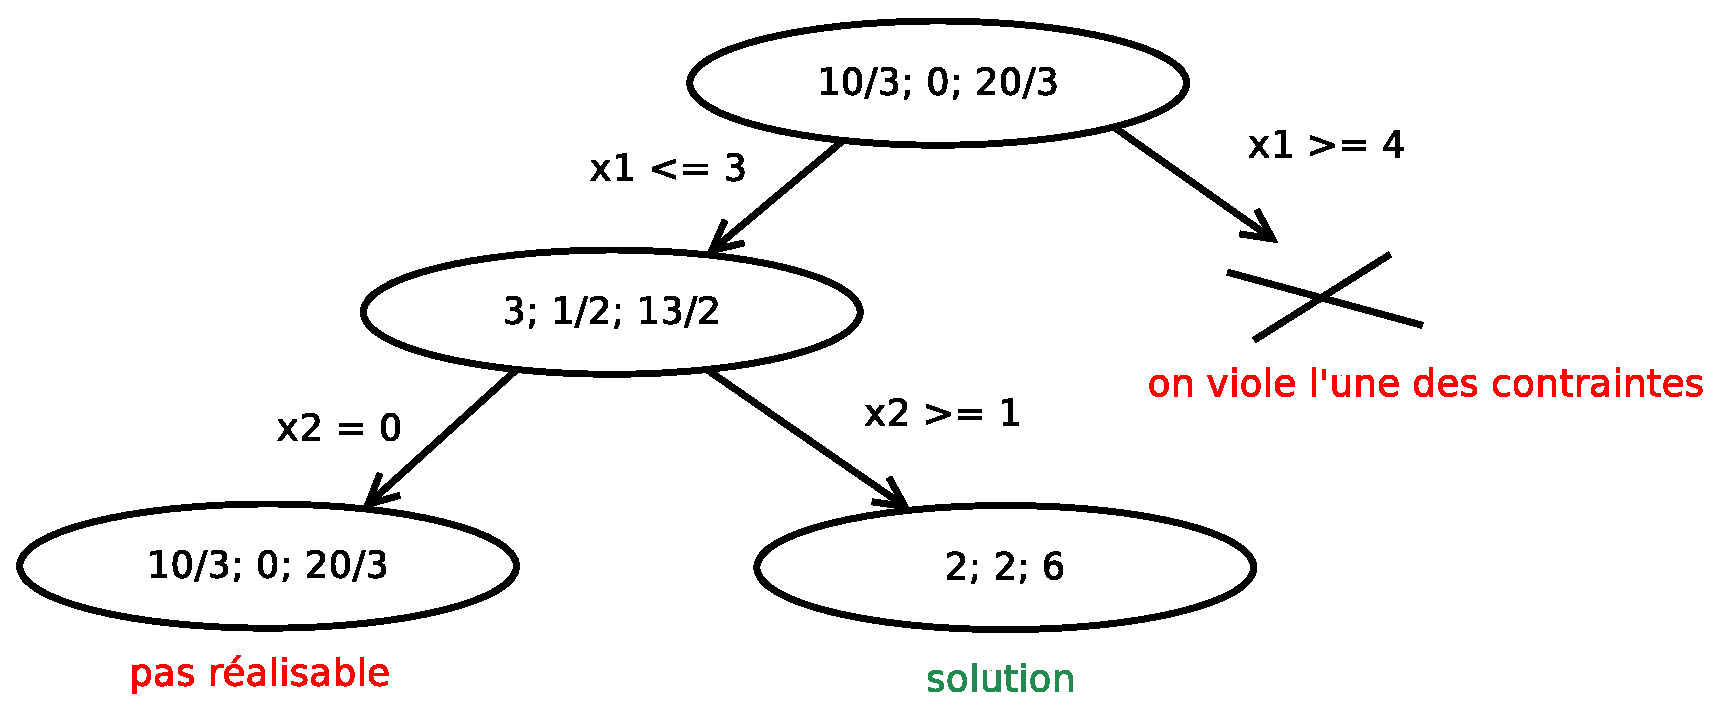
\includegraphics[height=60mm]{branchAndBound.eps}
\paragraph{Question 4, b) Branch and Cut}

Vous trouvez ci dessous les différents étapes des tableaux de la
méthode de Branch and Cut. \\
Les étapes intermédiaires sont les suivantes~:
\begin{itemize}
\item on commence par reprendre les résultats de la question
  concernant la résolution par le simplexe, puis l'on fixe la deuxième
  ligne, d'où $i = 2$.
\item $x_2$ et $x_4$ sont les variables qui ne sont pas en base. On
  peut donc écrire $\frac{2}{3} x_2 + \frac{1}{3} x_4 \geq
  \frac{1}{3}$.
\item Graphiquement, cela correspond à $x_1 \leq 3$ car on a 
\begin{equation}
\begin{cases}
2x_1 + 5x_2 + x_3  = 17 \\
3x_1 + 2x_2 + x_4  = 10 \\
\end{cases}
\\
\Rightarrow x_4  = 10 - 3x_1 - 2x_2 
\end{equation}
Ainsi, en remplaçant $x_4$ dans l'équation de l'item précédent, on a
\\
$\frac{2}{3}x_2 + \frac{1}{3}(10-3x_1-2x_2) \geq \frac{1}{3}$ \\
$\frac{2}{3}x_2 + \frac{10}{3} - x_1 - \frac{2}{3}x_2 \geq
\frac{1}{3}$ \\
$\frac{10}{3} - x_1 \geq \frac{1}{3}$ \\
$-x_1 \geq \frac{-9}{3} = -3$ \\
$\Rightarrow x_1 \leq 3$.
\item On rajoute la nouvelle contrainte obtenue dans notre tableau du
  simplexe, que nous résolvons alors par la méthode à deux phases.
\end{itemize}

TODO : étapes intermédiaires !!

\begin{table}[h!]	
\centering
	\begin{tabular}{|c|c|c|c|c|c|c|c|}
	\hline
      & c & 0 & 0 & 0 & 0 & 0 & -1 \\ 
      \cline{2-8}
       &  & $x_{1}$ & $x_{2}$  & $x_{3}$  & $x_{4}$ & $x_{5}$ & $y$ \\
       \hline
   0 & $x_{3}$  $=$ $\frac{31}{3}$ & 0 & $\frac{11}{3}$ & 1 & $\frac{-2}{3}$ & 0 & 0 \\
      \hline
	0 & $x_{1}$ $=$ $\frac{10}{3}$  & 1 & $\frac{2}{3}$ & 0 & $\frac{1}{3}$ & 0 & 0 \\
	  \hline
	  -1 & $y$ $=$ $\frac{1}{3}$  & 0 & $\frac{2}{3}$ & 0 & $\frac{1}{3}$ & -1 & 1 \\
	    \hline
	 $\frac{-1}{3}$ & Z($x$)$=$ 0 & 0 & $\frac{-2}{3}$ & 0 & $\frac{-1}{3}$ & 1 & 0\\
	  \hline
	\end{tabular}
\caption {Tableau 1 des coupes de Gomory}
\end{table}
\begin{table}[h!]	
\centering
	\begin{tabular}{|c|c|c|c|c|c|c|}
	\hline
      & c & 2 & 1 & 0 & 0 & 0 \\ 
      \cline{2-7}
       &  & $x_{1}$ & $x_{2}$  & $x_{3}$  & $x_{4}$ & $x_{5}$ \\
       \hline
   0 & $x_{3}$  $=$ $\frac{31}{3}$ & 0 & $\frac{11}{3}$ & 1 & $\frac{-2}{3}$ & 0 \\
      \hline
	2 & $x_{1}$ $=$ $\frac{10}{3}$  & 1 & $\frac{2}{3}$ & 0 & $\frac{1}{3}$ & 0 \\
	  \hline
	0 & $y$ $=$ $\frac{1}{3}$  & 0 & $\frac{2}{3}$ & 0 & $\frac{1}{3}$ & -1 \\
	  \hline
	 & Z($x$)$=$ $\frac{20}{3}$ & 0 & $\frac{-2}{3}$ & 0 & $\frac{-1}{3}$ & 1\\
	  \hline
	\end{tabular}
\caption {Tableau 1 de la méthode à deux phases}
\end{table}
\begin{table}[h!]	
\centering
	\begin{tabular}{|c|c|c|c|c|c|c|}
	\hline
      & c & 2 & 1 & 0 & 0 & 0 \\ 
      \cline{2-7}
       &  & $x_{1}$ & $x_{2}$  & $x_{3}$  & $x_{4}$ & $x_{5}$ \\
       \hline
   0 & $x_{3}$  $=$ $\frac{17}{2}$ & 0 & 0 & 1 & $\frac{-15}{6}$ & $\frac{11}{2}$ \\
      \hline
	2 & $x_{1}$ $=$ 3 & 1 & 0 & 0 & 0 & 1 \\
	  \hline
	1 & $x_{2}$ $=$ $\frac{1}{2}$  & 0 & 1 & 0 & $\frac{1}{2}$ & $\frac{-3}{2}$\\
	  \hline
	 & Z($x$)$=$ $\frac{13}{2}$ & 0 & 0 & 0 & $\frac{1}{2}$ & $\frac{1}{2}$\\
	  \hline
	\end{tabular}
\caption {Tableau 2 de la méthode à deux phases}
\end{table}

\pagebreak

\section{Partie pratique}

\subsection{Programmation dynamique}

Nous effectuerons ici les simulations du problème de la partition, du sac
à dos et du voyageur de commerce selon une implémentation
d'algorithmes basés sur de la programmation dynamique. Les programmes
seront écrits en langage C.

La programmation dynamique permet de trouver la solution optimale d'un
problème en combinant les solutions optimales de sous-problèmes de ce
problème.

\subsubsection{Sac à dos}

Nous avons commencé par nous intéresser au problème du sac à dos avant
partition car celui-ci est le plus général.

\paragraph{Modélisation}

Le problème du sac à dos se modélise en programmation linéaire de la
manière suivante~:

\begin{equation}
\begin{cases}
Max~z=\sum_{i=1}^nc_ix_i \\
\sum_{i=1}^na_ix_i \leq b \\
x_i \in\{0, 1\}, i=1\dots n\\
\end{cases}
\end{equation}

%Ainsi, nous prenons en paramètre~:
%\begin{itemize}
%\item le nombre $n$ d'objets sur lesquels nous
%désirons travailler, 
%\item le poids $b$ du sac que nous ne pouvons pas
%dépasser, 
%\item une variable binaire $x$, 
%\item un ensemble $C$ d'utilités à associer à chaque objet,
%\item un ensemble $A$ de poids à associer à chaque objet.
%\end{itemize}

\paragraph{Formules de programmation dynamique}

Les formules de programmation dynamique pour le problème du sac à dos
sont les suivantes~:
\begin{equation}
\begin{cases}
tab[0][w] = 0 \\
tab[i][j] = max(tab[i-1] [j], (tab[i-1] [j-poids[i]] + utilite[i])); \\
\end{cases}
\end{equation}

\paragraph{Implémentation en C}

Nous avons donc implémenté l'algorithme suivant (avec la fonction très
simple \textit{min} de calcul de minimum entre deux valeurs que nous
ne faisons pas figurer ici).

\begin{lstlisting}

int sacADos(int W, int* poids, int* utilite, int nbObjets){ 
//W represente la capacite max du sac

// tableau central de la programmation dynamique
int tab[nbObjets][W+1]; 
int w;

//initialisation de la table
for (w = 0; w < W + 1; w++){
  tab[0][w] = 0;
    }

//remplissage de la table selon les formules de la prog dyn
 int i, j;
 for (i = 1; i < nbObjets ; i++){
  for (j = 0; j < W + 1 ; j++) {
    if (j >= poids[i]) {
      tab[i][j] = max(tab[i-1] [j], 
(tab[i-1] [j-poids[i]] + utilite[i]));
    }
      else{
      tab[i][j] = tab[i-1] [j];
      }
    }
  }
//la valeur qui nous interesse
 printf(" poids : \%d \n", W);
 printf("meilleure solution (utilite) :
\%d \n", tab[nbObjets -1] [W]);
 return (tab[nbObjets -1] [W]);
}

\end{lstlisting}

\paragraph{Complexité théorique}

La complexité en temps de notre algorithme est en $O(nW)$. Il en va de
même pour la complexité mémoire.

\paragraph{Jeux de tests et temps d'exécution}

TODO

\subsubsection{Partition}

\paragraph{Modélisation}

Le problème de la partition se modélise de la manière suivante~:
\begin{equation}
\sum_{a \in A'} p(a)= \sum_{a \in A
    \backslash A'}p(a)
\end{equation}

\paragraph{Formules de programmation dynamique}

On se basera sur la récurrence suivante~:

\begin{equation}
\begin{cases}
tab[0] = 1; \\
si ( tab[j] == 1 ) {
       tab[j + poids[i]] = 1;
     } \\
\end{cases}
\end{equation}

\paragraph{Implémentation en C}

Nous présentons donc l'algorithme suivant, qui est une sorte de
restriction (cas particulier) de l'algorithme proposé pour la
résolution du problème du sac à dos~:

\begin{lstlisting}
int partition(int* poids, int nbObjets){ 


//calcul de la somme totale des poids
 int i, j;
int N = 0;
for(i = 0; i < nbObjets; i++ ) {N += poids[i];}

int tab[N]; 

//initialisation de la table de booleens

 tab[0] = 1;
 for(i = 1; i <= N; i ++ )  {tab[i] = 0;}


//remplissage de la table selon les formules de la prog dyn

 for(i = 0; i < nbObjets; i++ ){
   for(j = N - poids[i]; j >= 0; j-- ){
     if( tab[j] == 1 ) {
       tab[j + poids[i]] = 1;
     }
   }
 }

//la reponse qui nous interesse
 if(tab[N / 2] == 1){ 
   printf("vrai avec %d \n", N/2);
   }
 else{puts("faux");}

 return tab[N / 2];
}

\end{lstlisting}

\paragraph{Complexité théorique}

Soit $N$ la somme des poids.
La complexité en temps de notre algorithme est $O(nN)$.
La complexité mémoire est $O(N).$

\paragraph{Jeux de tests et temps d'exécution}

TODO

\subsubsection{Voyageur de commerce}

\paragraph{Modélisation}

Le problème du voyageur de commerce peut se modéliser de la manière
suivante~:


on se donne un graphe complet $K_n=(X,E)$ et on note $c_{ij}$ le poids
de l'arête $\{i,j\}$.
\begin{equation}
\begin{cases}
min \sum_{\{i, j\} \in E} c_{ij}.x_{ij} \\
\sum_{i=0}^n \sum_{j=0}^n x_{ij} = 1 \\
\forall (S, \bar{S}) \sum_{i \in S, j \in \bar{S}} x_{ij} \geq 1 \\
x_{ij} \in \{0, 1\} \\
\end{cases}
\end{equation}

\paragraph{Formules de programmation dynamique}

On note $C(S,i)$ la longueur d'une plus courte chaîne du sommet $0$ au
sommet $i$ qui passe une et une seule fois par tout sommet de $S$ et
qui n'utilise pas de sommet non dans $S$ autre que $i$. On a ainsi les
formules suivantes pour le problème du voyageur de commerce~:

\begin{equation}
\begin{cases}
C[S][i] = poids[0][i] \text{si S ne contient que $0$} \\
C[S][i] = min_{k \in S - \{ 0 \}} \{ C[S- \{ k \}][k] + poids[k][i]  \}
\end{cases}
\end{equation}

\paragraph{Implémentation en C}

TODO

\paragraph{Complexité théorique}

TODO

\paragraph{Jeux de tests et temps d'exécution}

TODO


\pagebreak

\subsection{Branch and bound}

Nous nous intéresserons au sein de cette section à la programmation de
la méthode de branch and bound pour résoudre le problème du voyageur
de commerce (tsp).

\subsubsection{Détermination de la solution initiale}

Dans cette partie, nous nous servirons de l'outil GLPK, et en
particulier de la syntaxe du langage Gnu MathProg. Pour le problème
présenté, un fichier .mod contenant la modélisation du problème est
créé ainsi qu'autant de fichiers .dat que de jeux de test. Nous nous
intéresserons à trois heuristiques en particulier.

\paragraph{Chaîne de poids le plus faible et ajout d'une arête pour le
  cycle}


\paragraph{Voisinage 2--opt}

\paragraph{Voisinage 3--opt}

\subsubsection{Programmation de l'algorithme $\frac{3}{2}$}

\paragraph{Principe de l'algorithme}

\paragraph{Complexité théorique}

\paragraph{Langage de programmation et bibliothèques}

\paragraph{Structures de données utilisées}

\paragraph{Principales fonctions}

\paragraph{Remarques}

\subsubsection{Tests}

\paragraph{Outils}

Nous utiliserons ici l'utilitaire console Unix time pour mesurer le
temps de calcul de nos programmes. Gprof sera également utilisé pour
une analyse un peu plus fine du temps de calcul (outil de profiling).

\paragraph{Tests de validité de notre programme}

\paragraph{Comparaison de l'efficacité de l'algorithme selon les
  trois heuristiques}


\paragraph{Comparaison entre la programmation dynamique et le branch and bound}

\subsection{Conclusion}

\end{document}
